\documentclass[runningheads]{llncs}

\usepackage[T1]{fontenc}
\usepackage{graphicx}
\usepackage{placeins}
\usepackage{booktabs}
\usepackage{multirow}
\usepackage{array}
\usepackage{amsfonts}
\usepackage{longtable}
\usepackage{listings}
\usepackage{url}
\usepackage{xcolor}
\renewcommand\UrlFont{\color{blue}\rmfamily}
\urlstyle{rm}
\emergencystretch=2em

\newcolumntype{L}[1]{>{\raggedright\arraybackslash}p{#1}}
\lstset{
    basicstyle=\ttfamily\scriptsize,
    breaklines=true,
    breakatwhitespace=false,
    columns=fullflexible,
    frame=single,
    keepspaces=true,
    showstringspaces=false
}

\title{ASB: Auditable Semantic Bottlenecks for\\
Reliable LLM-Generated Text Features}
\titlerunning{ASB for Reliable LLM-Generated Text Features}

\author{Huijie Xu\inst{1}\orcidID{0009-0006-7869-8113} \and
Zhiyu Zhu\inst{1}\orcidID{0009-0009-0231-4410} \and
Zhibo Jin\inst{1}\orcidID{0009-0003-0218-1941} \and
Hongyang Chen\inst{1}\orcidID{0009-0005-3240-4688} \and
Jianlong Zhou\inst{1}\orcidID{0000-0001-6034-644X}\thanks{Corresponding author.}}
\authorrunning{H. Xu et al.}

\institute{University of Technology Sydney, Sydney, NSW, Australia\\
\email{Huijie.Xu@student.uts.edu.au, Zhiyu.Zhu@student.uts.edu.au, Zhibo.Jin@student.uts.edu.au, Hongyang.Chen@student.uts.edu.au, Jianlong.Zhou@uts.edu.au}}

\begin{document}
\maketitle

\begin{abstract}
Large language models (LLMs) can turn text into human-readable variables, yet these prompt-conditioned measurements may encode label proxies and drift across extractors. We present Auditable Semantic Bottlenecks (ASB), which inserts a compact semantic layer before a classifier and makes the materialized feature matrix available for reliability analysis. We evaluate 20 binary concepts per dataset on SMS spam, sentiment, adverse drug event, and disaster tweet classification. Candidate concepts are proposed from training examples and screened for direct label leakage, duplicates, non-binary wording, source artifacts, and excessive specificity. ASB-LR achieves Macro-F1 scores of 0.937, 0.935, 0.758, and 0.807 across the four tasks. Human audits yield feature-level agreement of 0.841--0.917 and Cohen's $\kappa$ of 0.579--0.783, while prompt perturbations retain at least 0.959 matrix agreement. Provider changes produce task-level Macro-F1 spans of 0.016--0.058, and removing high-association concepts has its largest effect on SST-2 ($-0.158$). ASB links predictive semantic features to direct evidence about their construction, measurement, and reuse.
\keywords{semantic bottlenecks \and large language models \and reliability audit \and trustworthy AI}
\end{abstract}

\section{Introduction}

LLMs are increasingly used to generate features for text-mining pipelines: a prompt produces semantic variables for each text, and a conventional classifier operates on the resulting matrix. This intermediate representation is readable, but readability alone does not establish that its values are stable, non-leaking, or aligned with human judgments. Prompt wording and provider choice can change the matrix, while label-like shortcuts may remain even when the prompt never asks for the target label.

We study this measurement problem through Auditable Semantic Bottlenecks (ASB). Each text is encoded by 20 binary, human-readable questions organized into five semantic groups. Candidate questions are generated from training examples, screened under fixed rules, and frozen before held-out evaluation. Lightweight classifiers operate on the materialized matrix, whose values, coefficients, label associations, human agreement, prompt stability, and extractor sensitivity can all be measured directly. Prediction and reliability analysis thus use the same representation.

Our contributions are:

\begin{itemize}
    \item a reliability-audit framework centered on the LLM-generated feature matrix as a measurable object;
    \item a fixed 20-concept instantiation evaluated on four text-classification tasks against raw-text, embedding, fine-tuned transformer, and direct-LLM baselines; and
    \item an audit protocol covering direct leakage, label-proxy behavior, human agreement, prompt and schema sensitivity, cross-extractor transfer, and semantic interventions.
\end{itemize}

\section{Related Work}

Fine-tuned encoders such as BERT learn dense contextual representations from raw text~\cite{devlin2019bert}, while generative LLMs support zero- and few-shot prediction~\cite{brown2020language}. LLMs have also been used to produce lightweight representations, annotations, and training labels~\cite{liu2024llmembed,gilardi2023chatgpt,tan2024large,kumar2026large}. In contrast to treating these outputs as predictions or auxiliary supervision, ASB materializes a human-readable feature matrix and audits it before downstream use.

Post-hoc attribution assigns importance to model features~\cite{zhu2024enhancing,zhu2025narrowing}, whereas concept bottleneck models route predictions through variables that people can inspect or edit~\cite{koh2020concept}. Label-free and language-guided variants construct concepts from pretrained models~\cite{oikarinen2023label,yang2023language,tan2024interpreting,sun2025concept}; textual bottlenecks further support iterative concept discovery or completeness relative to a residual model~\cite{ludan2023interpretable,bhan2025towards}. ASB instead fixes a 20-question schema before held-out evaluation and evaluates the reliability of the generated measurements themselves.

ASB also relates to weak supervision and data programming~\cite{ratner2020snorkel} and to LLM-assisted taxonomy or supervision generation~\cite{wan2024tnt}. Prompt outputs can vary with wording and demonstrations~\cite{zhao2021calibrate,lu2022fantastically,chatterjee2024posix,zhou2024larger}, while general assessment frameworks combine utility, robustness, and interpretability at the model level~\cite{jin2023poster}. ASB focuses this assessment on direct leakage, train-only proxy strength, human agreement, prompt drift, and cross-extractor compatibility in the generated measurement layer.

\section{Methods}
\label{sec:methods}

\subsection{Problem Formulation}
\label{sec:problem-formulation}

For a binary text dataset $\mathcal{D}=\{(x_i,y_i)\}_{i=1}^{n}$, ASB factorizes prediction through an explicit semantic bottleneck:
\[
    g_{Q,e}(x_i)=z_i^e,\qquad h_\psi(z_i^e)=\hat{y}_i ,
    \qquad z_i^e\in\{0,1\}^{m}.
\]
Here $Q=\{q_1,\ldots,q_m\}$ is a fixed set of questions, $e=(\theta,p)$ combines the extractor model and prompt, and $h_\psi$ is a conventional classifier. For $Z^e=g_{Q,e}(X)\in\{0,1\}^{n\times m}$, downstream training minimizes
\[
    \min_{\psi} \frac{1}{|\mathcal{D}_{\mathrm{train}}|}
    \sum_{(x_i,y_i)\in\mathcal{D}_{\mathrm{train}}}
    \ell\!\left(h_\psi(z_i^e), y_i\right),
\]
with $Q$ and $e$ frozen before test evaluation. Reliability analysis evaluates $Z^e$ for stability, human alignment, label association, and direct leakage before interpreting downstream predictions.

\begin{figure}[!htbp]
\centering
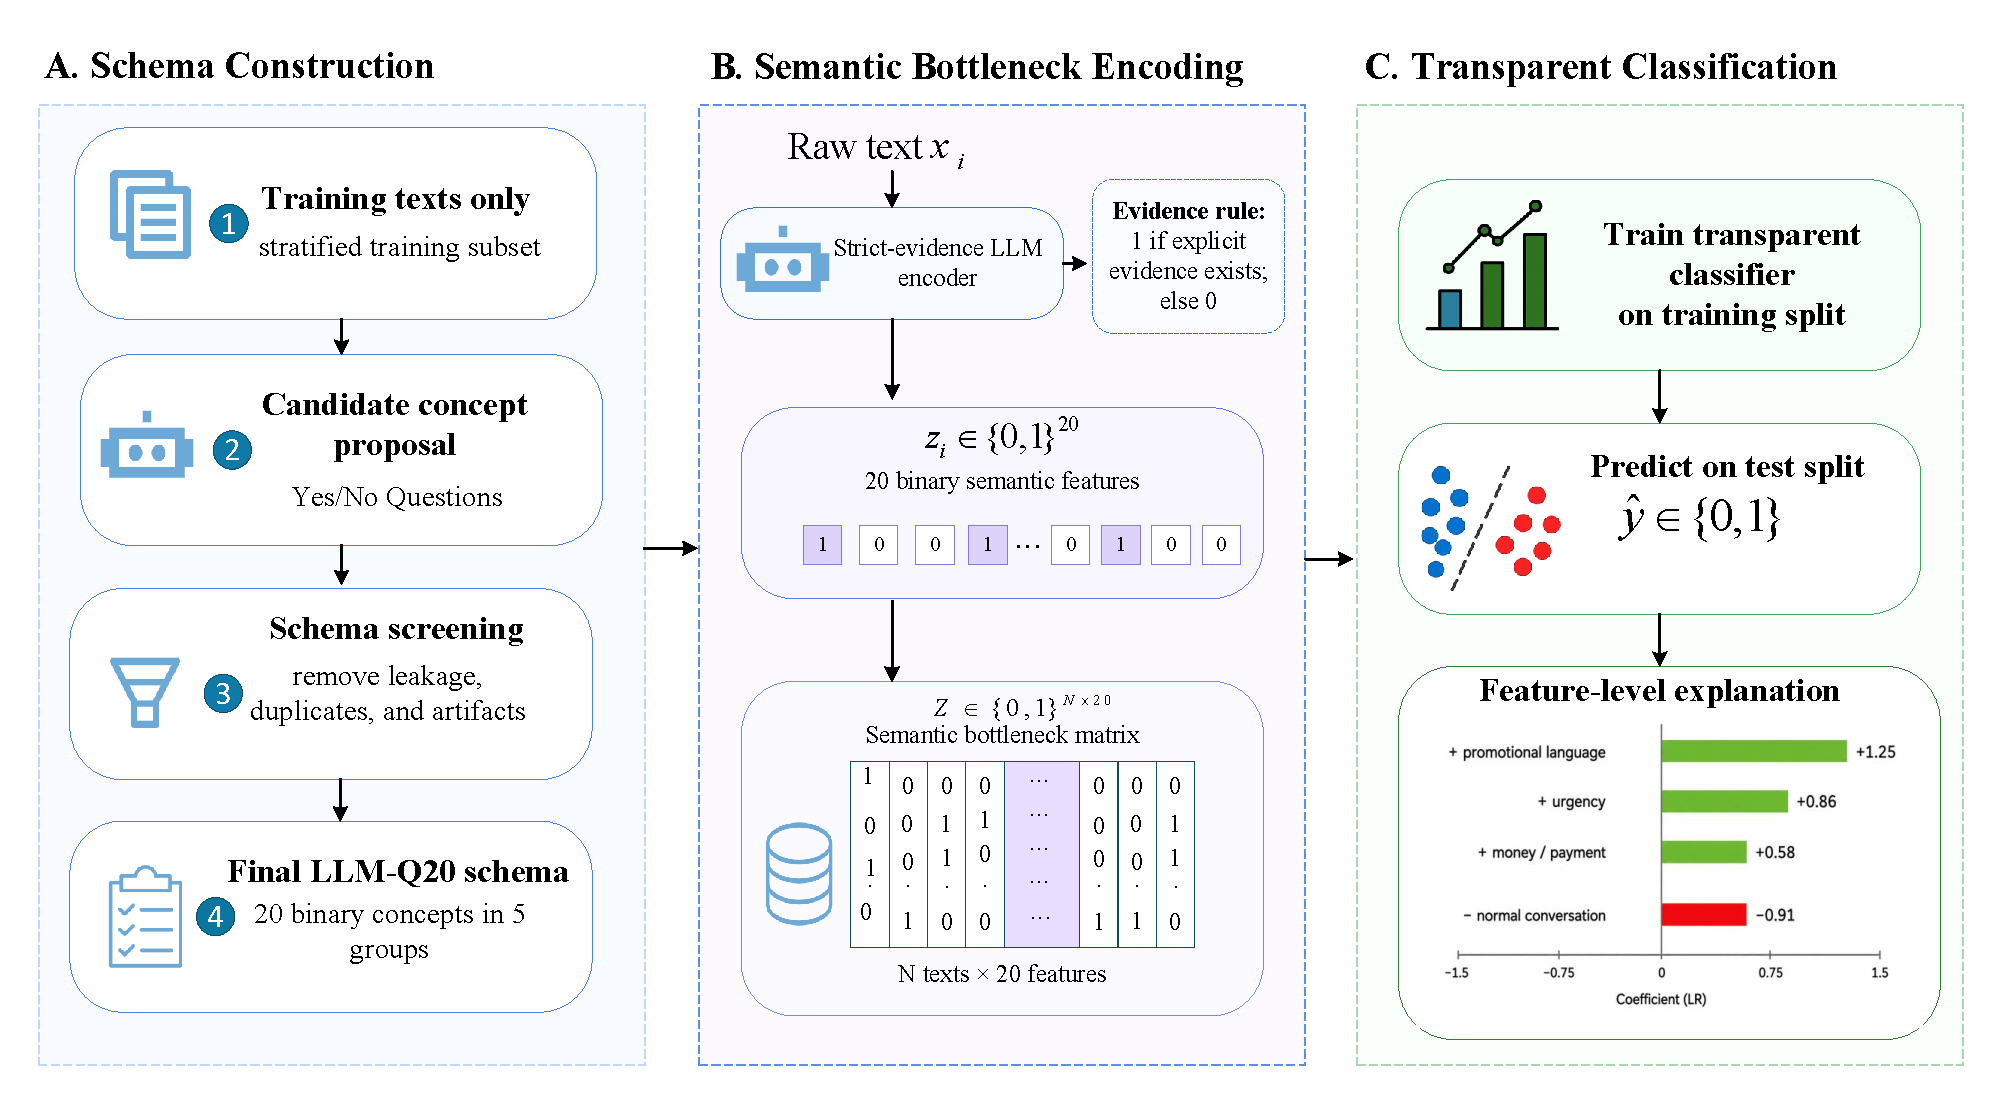
\includegraphics[width=0.86\textwidth]{figures/LLM-MINING.pdf}
\caption{ASB workflow from semantic extraction to downstream classification. Reliability tests operate directly on the generated feature matrix before downstream use.}
\label{fig:workflow}
\end{figure}

\subsection{ASB Semantic Encoding and Construction}
\label{sec:llm-encoding}

Given $Q$ and extractor $e$, a deterministic parser converts the JSON response into
\[
    z_i^{e}=(z_{i1}^{e},\ldots,z_{im}^{e})\in\{0,1\}^{m}.
\]
A value is 1 only when the text explicitly supports the feature; unsupported or uncertain answers map to 0. Invalid JSON, missing keys, and non-binary outputs trigger retry, while persistent failures remain extraction failures. Main matrices use DeepSeek V4 Flash at temperature 0 with thinking disabled and JSON formatting. Provider comparisons hold the schema, prompt, parser, and temperature fixed.

Before downstream training, an LLM proposes candidate questions from 500 stratified training examples. Gold labels may guide the discovery of intermediate concepts but never test-specific selection. A fixed checklist removes duplicates, direct label questions or synonyms, non-binary items, source artifacts, and instance-specific wording. The retained $m=20$ questions form a curated interpretability budget. Appendix~\ref{app:reproducibility} records the extraction contract and implementation settings; the complete question lists and prompt templates are part of the accompanying artifact.

\subsection{Downstream Models}
\label{sec:downstream-models}

The primary downstream classifier is ASB-LR, a logistic regression model over the semantic bottleneck:
\[
    h_\psi(z_i^e)=\sigma(\beta_0+\beta^\top z_i^e).
\]
It uses class-balanced weights and L2 regularization; $\beta$ assigns one signed coefficient to each concept. ASB-XGB provides a secondary nonlinear check. Hyperparameters are listed in Appendix~\ref{app:reproducibility}.

\subsection{Reliability Metrics}
\label{sec:reliability-metrics}

For extraction configurations $e$ and $e'$, representation-level matrix agreement is
\[
    A_Z(e,e') =
    \frac{1}{nm}
    \sum_{i=1}^{n}
    \sum_{j=1}^{m}
    \mathbf{1}[z_{ij}^{e}=z_{ij}^{e'}],
\]
Because sparse matrices can agree through shared zeros, we also compute positive agreement for feature $q_j$:
\[
    P_j(e,e') =
    \frac{2TP_j}{2TP_j + FP_j + FN_j}.
\]
where $TP_j$ is joint activation and $FP_j,FN_j$ are one-sided activations; inactive features under both configurations are excluded. We additionally report per-feature Cohen's $\kappa$, activation shifts, and prediction agreement. For each classifier error, the semantic edit diagnostic is
\[
    d_{\mathrm{cf}}(i) =
    \min_{z' \in \{0,1\}^{m}}
    \|z'-z_i^e\|_0
    \quad
    \mathrm{s.t.}\quad
    h_{\psi_e}(z') = y_i
\]
where $\|z'-z_i^e\|_0$ counts changed concepts and $\psi_e$ is fitted under $e$. The diagnostic measures distance in feature space; raw-text edit distance lies outside its definition.

\subsection{Label-Proxy and Human Audit Protocols}
\label{sec:label-proxy}

We distinguish direct leakage from association with observable textual evidence. Screening removes direct label questions and class synonyms; retained concepts are then characterized by training-set yes-rate gaps, mutual information, and coefficient direction under pre-specified descriptive cutoffs.

Two computer-science/software annotators independently assessed the same 100 held-out examples per dataset (seed 42; balanced where possible), producing 8,000 concept judgments each. Blind packets showed text, feature id, group, and question, but hid task labels and LLM outputs. Annotators marked 1, 0, or U (unclear); U values are excluded from scored denominators, and none occurred. Primary annotations define the ASB--human reference, while the second annotator estimates human--human reliability. The ADE results measure technical reproducibility by nonclinical annotators; clinical validation requires domain experts.

\subsection{Leakage Controls}

The schema, 20-feature budget, and prompts are fixed before held-out evaluation. Schema generation, proxy analysis, mutual-information ranking, and model fitting use training rows only; direct label questions are removed, and retained label-associated concepts are disclosed.

\section{Experiments}
\label{sec:experiments}

\subsection{Experimental Setup}

We evaluate ASB on four binary text classification tasks: SMS Spam \cite{almeida2011contributions}, SST-2 \cite{socher2013recursive}, ADE Corpus V2 \cite{gurulingappa2012extraction}, and Disaster Tweets \cite{kaggle_disaster_tweets}. These datasets cover spam detection, sentiment analysis, biomedical adverse-event detection, and social-media crisis detection. For each task, we remove empty texts, deduplicate normalized text strings, draw a stratified 5000-example sample, and create a fixed 4000/1000 stratified train/test split using random seed 42.

Each dataset uses five task-specific semantic groups with four binary questions per group. These cover positive and negative evidence, mechanisms, context, and counter-class cues without directly asking for the label. The complete 80-question inventory accompanies the artifact; Appendix~\ref{app:reproducibility} fixes the common extraction and modeling protocol.

\subsection{Baselines and Evaluation Protocol}

We compare ASB-LR with TF-IDF LR, frozen DistilBERT and RoBERTa embeddings with LR, fine-tuned DistilBERT~\cite{sanh2019distilbert}, and direct zero- and four-shot LLM classification. ASB-XGB is a secondary nonlinear check. ASB-LR is primary because its coefficients expose feature-level contributions. Direct LLM baselines use DeepSeek V4 Flash at temperature 0; four-shot runs use two training examples per label and seeds 1, 2, and 3, fixed before evaluation.

\subsection{RQ1: Are ASB Features Predictive?}

Table~\ref{tab:main-performance} compares held-out Macro-F1. ASB-LR tests how much predictive signal can be retained in only 20 inspectable binary features.

ASB-LR reaches Macro-F1 scores of 0.9373, 0.9349, 0.7577, and 0.8073 on SMS Spam, SST-2, ADE, and Disaster Tweets, respectively. The SST-2 result is within 0.0125 of four-shot direct classification and exceeds both embedding baselines and fine-tuned DistilBERT on this split. Across all four tasks, the 20-feature matrix remains directly inspectable and reusable by conventional classifiers.

\begin{table}[!tbp]
\centering
\caption{Held-out Macro-F1. Values are point estimates or means over seeds where applicable.}
\label{tab:main-performance}
\setlength{\tabcolsep}{5.0pt}
\resizebox{\textwidth}{!}{%
\begin{tabular}{lcccccc}
\toprule
Dataset & TF-IDF LR & RoBERTa LR & DistilBERT FT & LLM 0-shot & LLM 4-shot & ASB-LR (ours) \\
\midrule
SMS Spam & 0.9676 & 0.9749 & 0.9795 & 0.9420 & 0.9668 & 0.9373 \\
SST-2 & 0.7669 & 0.8961 & 0.8998 & 0.9574 & 0.9479 & 0.9349 \\
ADE & 0.7623 & 0.7783 & 0.8570 & 0.7019 & 0.6898 & 0.7577 \\
Disaster Tweets & 0.7720 & 0.8290 & 0.8133 & 0.7711 & 0.8234 & 0.8073 \\
\bottomrule
\end{tabular}
}
\end{table}

\subsection{RQ2: Do ASB Concepts Support Feature-Level Audit?}

We audit the retained concepts along two axes: training-only label association and agreement with blind human judgments on held-out examples. Direct label questions are removed during schema screening.

Table~\ref{tab:proxy-summary} separates proxy strength from semantic role. Each schema contains observable high-association cues together with mechanistic and counter-class evidence, making the predictive evidence visible at feature level.

\begin{table}
\centering
\caption{Train-only label-proxy and semantic-role summary for retained ASB features. Proxy-strength columns partition the 20 features by descriptive training-label association cutoffs; role columns partition the same 20 features by audit role.}
\label{tab:proxy-summary}
\begin{tabular}{lrrrrrr}
\toprule
Dataset & High & Medium & Low & Class proxy & Mechanism & Counter \\
\midrule
SMS Spam & 9 & 8 & 3 & 6 & 10 & 4 \\
SST-2 & 7 & 5 & 8 & 3 & 4 & 13 \\
ADE & 2 & 4 & 14 & 2 & 12 & 6 \\
Disaster Tweets & 6 & 8 & 6 & 5 & 10 & 5 \\
\bottomrule
\end{tabular}
\end{table}

We remove every feature meeting a pre-specified training-only cutoff (absolute class-conditional yes-rate gap $\geq 0.50$ or mutual information $\geq 0.10$) and refit without changing the split or hyperparameters. Removing 9, 7, 2, and 6 features changes Macro-F1 from 0.9373 to 0.8919, 0.9349 to 0.7769, 0.7577 to 0.7238, and 0.8073 to 0.7484, respectively. The drops quantify the predictive signal carried by the disclosed high-association concepts, with the largest dependence on SST-2 ($-0.1580$).

Table~\ref{tab:concept-audit} reports the held-out concept-level audit. Primary human labels are the audit reference for ASB--human agreement and $\kappa$. Across datasets, ASB--human agreement ranges from 0.8410 to 0.9165, with $\kappa$ from 0.5791 to 0.7828. The low false-positive rates indicate that the strict extractor rarely activates unsupported concepts. The higher false-negative rates, especially on SST-2 and Disaster Tweets, show that it often under-activates subjective or context-dependent concepts.

A second annotator labeled the same packets. Human--human agreement ranges from 0.8665 to 0.9285, with $\kappa$ from 0.6604 to 0.8241. Both annotators have computer-science/software backgrounds, so the ADE figures characterize technical reproducibility; expert biomedical agreement remains to be established.

\begin{table}
\centering
\caption{Concept-level human audit of ASB feature values. Each dataset uses 100 held-out examples and 20 feature judgments per example. Inter-human columns compare the primary and second human annotators; ASB false-positive and false-negative rates are computed relative to the primary human labels.}
\label{tab:concept-audit}
\setlength{\tabcolsep}{3.5pt}
\begin{tabular}{@{}lrrrrrr@{}}
\toprule
Dataset &
\begin{tabular}[c]{@{}c@{}}ASB\\agree\end{tabular} &
\begin{tabular}[c]{@{}c@{}}ASB\\$\kappa$\end{tabular} &
\begin{tabular}[c]{@{}c@{}}Inter-human\\agree\end{tabular} &
\begin{tabular}[c]{@{}c@{}}Inter-human\\$\kappa$\end{tabular} &
ASB FP & ASB FN \\
\midrule
SMS Spam & 0.9155 & \textbf{0.7828} & \textbf{0.9285} & \textbf{0.8241} & 0.0253 & 0.2313 \\
SST-2 & 0.8410 & 0.6470 & 0.8655 & 0.7059 & \textbf{0.0133} & 0.3789 \\
ADE & \textbf{0.9165} & 0.7817 & 0.8850 & 0.7053 & 0.0304 & \textbf{0.2224} \\
Disaster Tweets & 0.8450 & 0.5791 & 0.8665 & 0.6604 & 0.0221 & 0.4681 \\
\bottomrule
\end{tabular}
\end{table}

Replacing all 20 values by human judgments on the audited examples corrects four SMS errors without introducing one and changes the number correct by $-1$, $-5$, and $-6$ on SST-2, ADE, and Disaster Tweets. An overdose relation and an ``Outdoor Siren Test'' illustrate cases where human-valued features cross a boundary learned from extractor-valued training data. Effective intervention therefore depends on compatibility between annotator semantics and the representation used to fit the classifier.

\subsection{RQ3: Prompt Stability and Extractor Sensitivity}

We separate prompt from extractor sensitivity. Under prompt perturbations with the same extractor and schema (Figure~\ref{fig:rq3-stability-sensitivity}a), minimum matrix agreement is 0.9588, minimum mean per-feature $\kappa$ is 0.8414, and minimum prediction agreement is 0.9450.

With schema and prompt fixed but provider changed (Figure~\ref{fig:rq3-stability-sensitivity}b), the Macro-F1 span ranges from 0.0155 on Disaster Tweets to 0.0575 on ADE, quantifying extractor-induced drift under a fixed measurement specification.

A stricter test trains on one provider's matrix and evaluates another provider's matrix without refitting. For the DeepSeek-source model, mean Macro-F1 changes across other extractors are $+0.0143$, $+0.0007$, $+0.0018$, and $-0.0041$ across the four tasks, with a worst target change of $-0.0281$. Transfer is asymmetric: among 48 off-diagonal directions, the largest drop is $-0.0790$ for GPT-4.1-mini-trained ADE evaluated on Gemini features. The artifact includes all 64 source--target combinations.

\begin{figure}[!tbp]
\centering
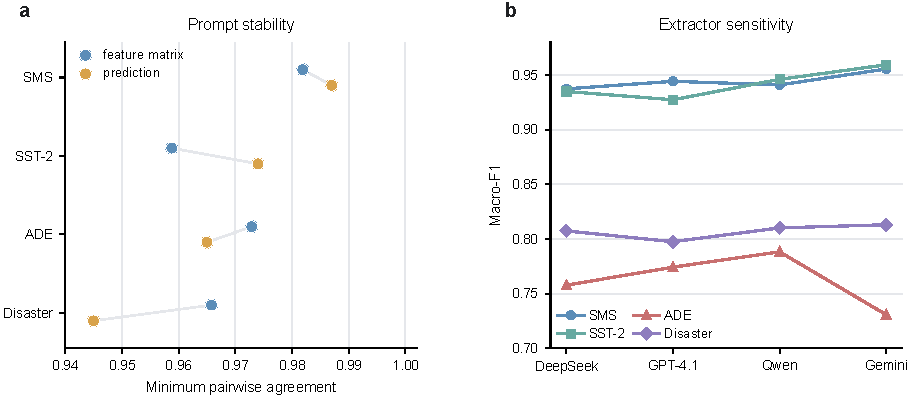
\includegraphics[width=\textwidth]{figures/rq3_stability_sensitivity.pdf}
\caption{Prompt and extractor sensitivity diagnostics. (a) Minimum pairwise agreement under prompt perturbations for feature matrices and downstream predictions. (b) ASB-LR Macro-F1 when the fixed schema and extraction prompt are run with different LLM extractors.}
\label{fig:rq3-stability-sensitivity}
\end{figure}

\subsection{RQ4: How Sensitive Is ASB to Schema Choice?}

For each dataset, we generate a training-only 40-concept candidate pool, select an alternative 20-concept schema under the same rules, and re-extract all 5000 rows with the same extractor. Table~\ref{tab:schema-summary} shows gains on SMS Spam and Disaster Tweets and reductions on SST-2 and ADE, directly measuring sensitivity to concept choice under a fixed construction protocol.

We fix 20 concepts before evaluation as the representation's interpretability budget. Train-only mutual-information selection (Figure~\ref{fig:asb-results-summary}a) shows that smaller subsets sometimes preserve performance, but the best size varies by task.

We also retain all 100 fixed-seed random 20-concept panels drawn per dataset from the materialized 40-feature union. Mean $\pm$ standard-deviation Macro-F1 is $0.9506\pm0.0104$, $0.9216\pm0.0180$, $0.7541\pm0.0243$, and $0.8130\pm0.0081$; ADE reaches a minimum of 0.6281. This sampling distribution characterizes variation within the fixed 40-feature pool; independent schema regeneration remains a separate source of variation.

\begin{table}[!htbp]
\centering
\caption{Schema-sensitivity summary. Alternative schemas are selected from training-only candidate pools using the same screening rules. Lexical overlap is mean maximum token-level Jaccard similarity; feature correlation is mean maximum absolute correlation over paired 5000-row feature matrices.}
\label{tab:schema-summary}
\begin{tabular}{lccccc}
\toprule
Dataset & Orig. Macro-F1 & Alt. Macro-F1 & $\Delta$ Macro-F1 & Lex. overlap & Feat. corr. \\
\midrule
SMS Spam & 0.9373 & 0.9676 & +0.0302 & 0.2351 & 0.6789 \\
SST-2 & 0.9349 & 0.8889 & -0.0460 & 0.2346 & 0.5261 \\
ADE & 0.7577 & 0.7533 & -0.0044 & 0.2351 & 0.6307 \\
Disaster Tweets & 0.8073 & 0.8194 & +0.0121 & 0.3838 & 0.6549 \\
\bottomrule
\end{tabular}
\end{table}
\FloatBarrier

\subsection{RQ5: Feature-Budget and Error-Intervention Diagnostics}

Figure~\ref{fig:asb-results-summary} places two feature-space diagnostics side by side: train-only mutual-information feature selection and semantic edits for ASB-LR test errors. The edit diagnostic counts the minimum number of binary feature edits needed to flip each erroneous prediction to the true label.

\begin{figure}[!htbp]
\centering
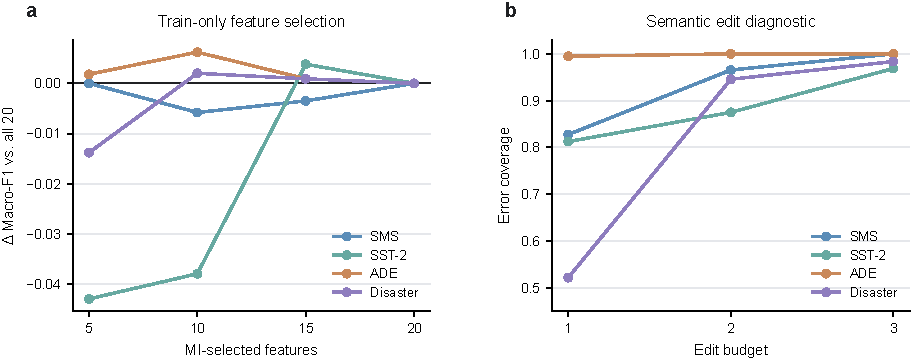
\includegraphics[width=0.92\textwidth]{figures/asb_results_summary.pdf}
\caption{Feature-budget and semantic-intervention diagnostics. (a) Change in ASB-LR Macro-F1 under train-only mutual-information selected subsets. (b) Fraction of ASB-LR test errors flipped within one, two, or three binary feature edits.}
\label{fig:asb-results-summary}
\end{figure}

The diagnostic localizes errors in feature space, while raw-text rewrite distance lies outside its definition. Median edit distance is 1.0 for all tasks, and three-edit coverage ranges from 0.9688 to 1.0000. Disaster Tweets is the hardest one-edit case, consistent with figurative and event-grounding ambiguity.
\FloatBarrier

\section{Discussion and Conclusion}

ASB turns LLM feature extraction into a measurable stage of a text-classification pipeline by making the generated semantic matrix the unit of analysis. Across four tasks, the same 20-variable representation is used to fit classifiers, compare human judgments, measure prompt and provider drift, and perform targeted feature interventions. These concepts achieve Macro-F1 scores of 0.758--0.937, while disagreements can be traced to individual features before the representation is reused.

The audits identify distinct sources of variation. SST-2 has the largest proxy-removal effect ($-0.1580$ Macro-F1), whereas ADE records both the largest cross-extractor drop ($-0.0790$) and the lowest resampled-panel score (0.6281). Transfer direction matters because classifiers are fitted to the activation patterns of a particular extractor. ASB false negatives also exceed false positives on every task: the strict evidence rule under-activates subjective, figurative, and relation-level concepts more often than it asserts unsupported ones. A ternary representation could preserve unclear evidence that is currently stored as 0.

\paragraph{Scope and responsible use.}
The experiments cover binary text classification with 20 binary features. Schema construction includes rule-guided author screening, ADE agreement is measured by nonclinical annotators, and the 100-panel analysis samples from one independently generated 40-candidate pool per task. Extending the evaluation to multi-label tasks, long documents, clinical experts, and independently regenerated schemas would test additional operating settings. Biomedical or disaster-monitoring use requires expert review, disclosure of LLM-generated features, and provider-drift monitoring. The artifact will release questions, prompts, parsing rules, seeds, audit formats, and redistributable cached outputs.

Together, the predictive and audit results show that a compact semantic bottleneck can retain useful task signal while exposing how concept choice, extractor behavior, and human interpretation shape downstream predictions.

\appendix
% !TEX root = ASB.tex
\section{Additional Experimental Details}
\label{app:reproducibility}

\paragraph{Data and schema boundary.}
For every task, empty texts are removed and normalized texts are deduplicated before drawing a stratified 5000-example sample and a fixed 4000/1000 split (seed 42). ChatGPT-5.5 proposes candidates from 500 stratified training examples; held-out texts are never shown. The same screening checklist removes duplicates, direct label questions or synonyms, non-binary items, source artifacts, and instance-specific wording, leaving five groups of four questions. Proxy analysis, mutual-information selection, and model fitting use training rows only.

\begin{table}[!htbp]
\centering
\caption{Semantic coverage of each fixed 20-question schema; every group contains four questions.}
\label{tab:compact-schema-groups}
\small
\setlength{\tabcolsep}{4pt}
\begin{tabular}{@{}L{2.2cm}L{9.0cm}@{}}
\toprule
Dataset & Semantic groups \\
\midrule
SMS Spam & deception; money; urgency; requested action; personal and normal context \\
SST-2 & positive sentiment; negative sentiment; aspect evaluation; uncertainty and irony; recommendation \\
ADE & medication; clinical event; causality and temporality; negation and uncertainty; non-ADE context \\
Disaster Tweets & disaster event; grounding; severity and damage; emergency response; figurative and non-disaster use \\
\bottomrule
\end{tabular}
\end{table}

\paragraph{Strict extraction contract.}
The system prompt requires one JSON object containing exactly the 20 feature identifiers and binary values, with 1 used only for explicitly supported evidence and 0 for absent, unsupported, or unclear evidence. A dataset-specific guard forbids direct classification as spam/ham, positive/negative, ADE/non-ADE, or real/non-disaster. The parser normalizes Boolean and yes/no values, retries invalid JSON, missing identifiers, and non-binary values, and records persistent failures rather than silently mapping them to zero.

The invariant core of the system prompt is:
\begin{lstlisting}
You convert texts into semantic yes/no features.
Return JSON only. Do not include markdown, explanations, or extra keys.
For every feature id, return 1 for yes and 0 for no.
If the answer is unclear or not supported by the text, return 0.
{task_guard}
\end{lstlisting}
The user message supplies the text and the 20 identifier--question pairs, then requires exactly those identifiers in the returned object.

\subsection{Implementation and Supporting Analyses}

\begin{table}[!htbp]
\centering
\caption{Fixed extraction, modeling, and audit settings.}
\label{tab:compact-reproducibility}
\small
\setlength{\tabcolsep}{4pt}
\begin{tabular}{@{}L{2.7cm}L{8.5cm}@{}}
\toprule
Component & Setting \\
\midrule
ASB extraction & DeepSeek V4 Flash; strict-evidence prompt; temperature 0; thinking disabled; JSON response. Provider tests additionally use GPT-4.1 mini, Qwen Plus, and Gemini 2.5 Flash with the same schema, prompt, parser, and temperature. \\
TF-IDF LR & Lowercased word unigrams/bigrams; minimum document frequency 2; L2 LR, $C=1$, \texttt{lbfgs}, class-balanced weights, maximum 1000 iterations. \\
Embedding LR & \texttt{distilbert-base-uncased} or \texttt{roberta-base}; attention-mask mean pooling; maximum length 128; batch size 64; the same LR settings. \\
DistilBERT tuning & \texttt{distilbert-base-uncased}; maximum length 128; AdamW, learning rate $2\times10^{-5}$, no scheduler; 3 epochs; batch size 8. \\
ASB models & LR uses the settings above over 20 binary features. XGBoost uses 100 trees, depth 3, learning rate 0.1, full row/column sampling, log-loss, and train-imbalance weighting. \\
Repeated runs & Seeds 1, 2, and 3 where applicable. Four-shot LLM classification uses two training examples per label; deterministic cached configurations are not treated as uncertainty estimates. \\
Human audit & Two blind annotators independently score the same 100 held-out texts per task and all 20 concepts as 0, 1, or U; U is excluded from scored denominators. \\
\bottomrule
\end{tabular}
\end{table}

Table~\ref{tab:compact-reproducibility} records the implementation settings, and Table~\ref{tab:compact-repeatability} separates seeded variability from fixed-pipeline results. Fine-tuning and four-shot prompting vary across three seeds; daggers identify operating points that reuse a fixed split, cached representation, temperature-0 output, and/or deterministic solver. Across the four tasks, ASB-XGB differs from ASB-LR by at most 0.0033 Macro-F1.

\begin{table}[!htbp]
\centering
\caption{Macro-F1 repeatability and nonlinear-model check. Stochastic entries are mean $\pm$ standard deviation over three seeds.}
\label{tab:compact-repeatability}
\small
\setlength{\tabcolsep}{5pt}
\begin{tabular}{@{}lcccc@{}}
\toprule
Dataset & DistilBERT FT & LLM 4-shot & ASB-LR & ASB-XGB \\
\midrule
SMS Spam & $0.9795\pm0.0096$ & $0.9668\pm0.0148$ & $0.9373^{\dagger}$ & $0.9393^{\dagger}$ \\
SST-2 & $0.8998\pm0.0018$ & $0.9479\pm0.0041$ & $0.9349^{\dagger}$ & $0.9349^{\dagger}$ \\
ADE & $0.8570\pm0.0354$ & $0.6898\pm0.0535$ & $0.7577^{\dagger}$ & $0.7610^{\dagger}$ \\
Disaster Tweets & $0.8133\pm0.0066$ & $0.8234\pm0.0090$ & $0.8073^{\dagger}$ & $0.8066^{\dagger}$ \\
\bottomrule
\end{tabular}
\end{table}

Table~\ref{tab:compact-stress-tests} reports proxy removal, cross-extractor transfer without refitting, panel resampling from the materialized 40-feature pool, and human replacement on the audit packets. The four columns measure construct selection, measurement stability, and downstream compatibility under their stated conditions.

\begin{table}[!htbp]
\centering
\caption{Supporting stress-test summary. Transfer values are Macro-F1 changes; human net is errors fixed minus errors introduced.}
\label{tab:compact-stress-tests}
\small
\setlength{\tabcolsep}{3.5pt}
\resizebox{\textwidth}{!}{%
\begin{tabular}{@{}lrrrrrr@{}}
\toprule
Dataset & Proxy-removal $\Delta$ & DeepSeek mean transfer $\Delta$ & Global worst transfer $\Delta$ & Panel mean $\pm$ SD & Panel minimum & Human net \\
\midrule
SMS Spam & $-0.0455$ & $+0.0143$ & $-0.0293$ & $0.9506\pm0.0104$ & 0.9062 & $+4$ \\
SST-2 & $-0.1580$ & $+0.0007$ & $-0.0323$ & $0.9216\pm0.0180$ & 0.8696 & $-1$ \\
ADE & $-0.0339$ & $+0.0018$ & $-0.0790$ & $0.7541\pm0.0243$ & 0.6281 & $-5$ \\
Disaster Tweets & $-0.0590$ & $-0.0041$ & $-0.0245$ & $0.8130\pm0.0081$ & 0.7916 & $-6$ \\
\bottomrule
\end{tabular}%
}
\end{table}

SST-2 has the largest proxy-removal change, whereas ADE has the largest cross-extractor drop and the lowest resampled-panel score. Human replacement improves SMS and reduces accuracy on the other tasks. These outcomes show that concept selection, extractor choice, and annotator semantics can each alter downstream behavior.

\paragraph{Artifact boundary.}
The package contains all 80 questions, prompts, split identifiers, parsed matrices, audit templates, detailed tables, figure data, and redistributable cached outputs; credentials, private logs, and restricted data are excluded.


\bibliographystyle{splncs04}
\bibliography{references}

\end{document}
